\documentclass{article}

\usepackage[margin=1in]{geometry}
\usepackage{listings}
\usepackage{color}
\usepackage{graphicx}
\usepackage{float}

\definecolor{dkgreen}{rgb}{0,0.6,0}
\definecolor{gray}{rgb}{0.5,0.5,0.5}
\definecolor{mauve}{rgb}{0.58,0,0.82}

\lstset{frame=tb,
	language=C,
	aboveskip=3mm,
	belowskip=3mm,
	showstringspaces=false,
	columns=flexible,
	basicstyle={\small\ttfamily},
	numbers=left,
	numberstyle=\color{gray},
	keywordstyle=\color{blue},
	commentstyle=\color{dkgreen},
	stringstyle=\color{mauve},
	breaklines=true,
	breakatwhitespace=true,
	tabsize=4
}

\title{Lab 6: Stepper Motor}
\date{November 06, 2017}
\author{Matthew Friedman 861151348\\Souradeep Bhattacharya 861105938\\EE128 Section: 021}
\begin{document}
	\maketitle
	\section*{Abstract}
	The objective of this lab was to become familiar with the control of stepper motors. We create a program to control a stepper motor's direction and speed based off of two input switches.
	\section*{Experimental System Specification}
	Create a system using the L298N that will control the direction (clock wise and counter-clockwise) and the speed of the motor (22.5 degrees per second and 90 degrees per second) based on the input of two switches.
	\section*{Block Diagram}
	\begin{figure}[H]
		\centering
		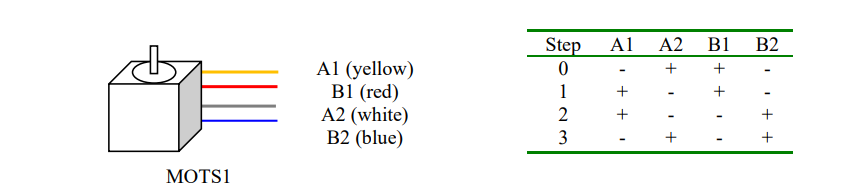
\includegraphics[width=1\textwidth]{StepperMotorBlock}
		\caption{Stepper motor pin block diagram.}
	\end{figure}
	\begin{figure}[H]
		\centering
		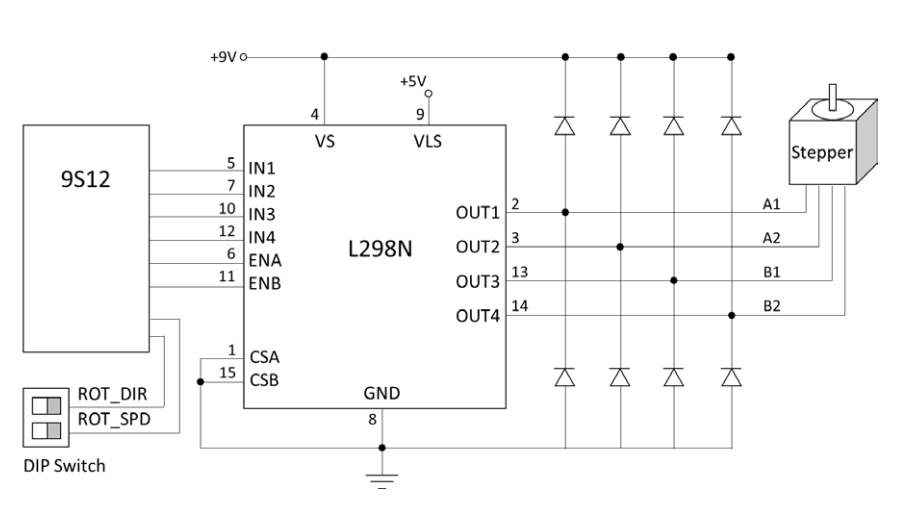
\includegraphics[width=1\textwidth]{OverallBlockDiagram}
		\caption{Overall System block diagram}
	\end{figure}
	\section*{Detailed Schematic}
	\begin{figure}[H]
		\centering
		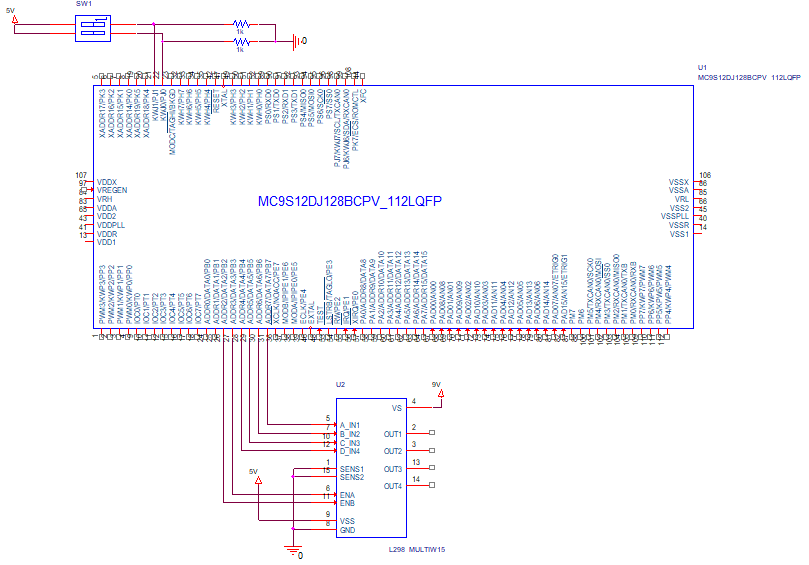
\includegraphics[width=1\textwidth]{Schematic}
		\caption{System Schematic}
	\end{figure}
	\begin{figure}[H]
		\centering
		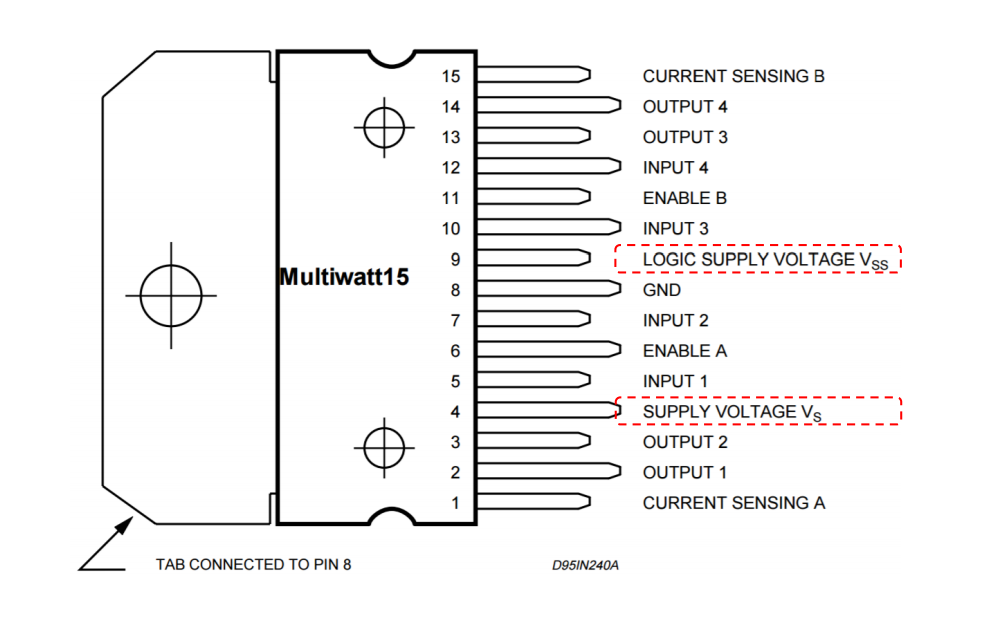
\includegraphics[width=1\textwidth]{L298Pinout}
		\caption{L298N Pinout}
	\end{figure}
	\begin{figure}[H]
		\centering
		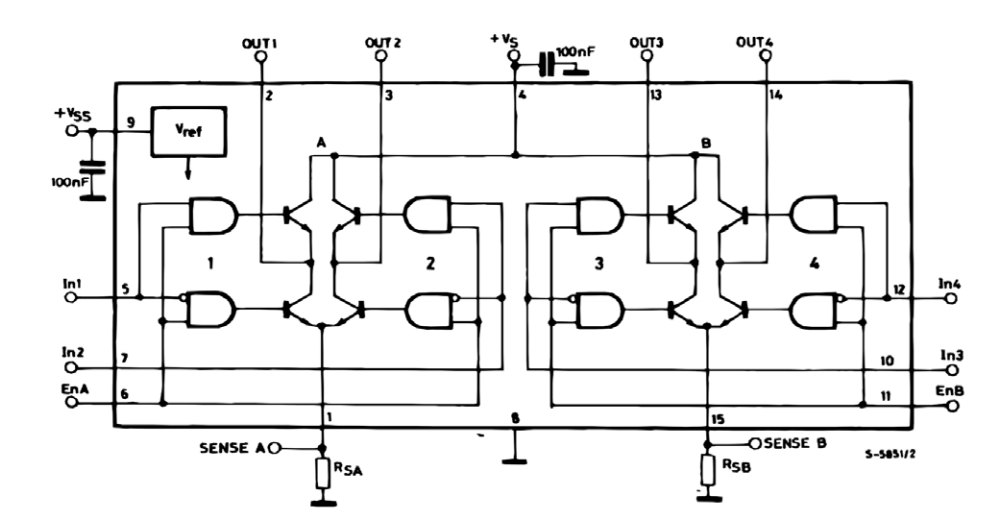
\includegraphics[width=1\textwidth]{L298BlockDiagram}
		\caption{L298N Internal Block Diagram}
	\end{figure}
	\section*{High Level Description of Software}
	This program reads the states of two switches and determines the speed of rotation (0: 22.5 degrees per second, 1: 90 degrees per second.) and the direction of rotation (0: clockwise, 1: counter-clockwise). It then controls an L298N to drive a stepper motor.
	\section*{Program Listing}
	\begin{lstlisting}
	#include <hidef.h>      /* common defines and macros */
	#include "derivative.h"      /* derivative-specific definitions */	
	
	unsigned long i;
	char rot_dir = 0; //PA0
	char rot_spd = 0; //PA1
	unsigned long speed_val = 30000;
		
	void main(void)   //OUT1=PB0 OUT2=PB1 OUT3=PB2 OUT4=PB3
	{
		DDRB = 0xFF; //output for stepper
		DDRA = 0x00; //input for switch
		PORTB = 0x30;
		
		while (1) 
		{    
			//check switch
			rot_dir = PORTA & 0x01;
			rot_spd = PORTA & 0x02;
			
			//change speed
			if(rot_spd) 
			{
				speed_val = 7500;//faster
			} 
			else 
			{
				speed_val = 30000;//slower
			}
		
			//change direction
			if(rot_dir) 
			{      
				//step CW
				PORTB = 0x36;
				for (i = 0; i < speed_val; i++);
				
				PORTB = 0x35;
				for (i = 0; i < speed_val; i++);
				
				PORTB = 0x39;
				for (i = 0; i < speed_val; i++);
				
				PORTB = 0x3A;
				for (i = 0; i < speed_val; i++);
			} 
			else 
			{
				//step CCW
				PORTB = 0x3A;
				for (i = 0; i < speed_val; i++);
				
				PORTB = 0x39;
				for (i = 0; i < speed_val; i++);
				
				PORTB = 0x35;
				for (i = 0; i < speed_val; i++);
				
				PORTB = 0x36;
				for (i = 0; i < speed_val; i++); 
			}
		}
	}
	\end{lstlisting}
	\section*{Technical Problems}
	\paragraph*{Program wasn't working} We had forgotten to change a parameter in the burner for the HS912.
	\section*{Answers to Questions}
	\subsection*{Prelab Question}
	It can not change it instantly. This is because of the fact that each coil is an inductor and to conduct an instantaneous change in current would require an infinite voltage over the inductor coil. It can change direction only if the next coil has not been energized yet. Then changing direction is simply the result of activating another coil.
	\subsection*{Lab Questions}
	We experienced the motor stalling only when we did not trigger the coils correctly. It could also happen if the program switched too quickly resulting in stalling because the coils would not be energized fast enough to move the motor.
	\section*{Conclusion}
	In this lab we were able to successfully control the stepper motor. We did this lab with software loops, we could have also done it with the hardware timer.
\end{document}